\chapter{Armas.}
%=================================================
\section{Nombre: Caracola.} \label{Arma:Caracola}
\subsection{Descripción}
Esta arma con forma de cenzontle contiene el alma de uno dentro, lo que le permita generar todo tipo de sonidos. El sonido que produce se ve materializado como energía luminosa que puede atacar a los enemigos y proteger a su portador al generar una barrera.
\subsection{Imagen}

\subsection{Portador}
Malinalli.
%=================================================
\section{Nombre: Atardecer de venus.}\label{Arma:BaculoXolotl}
	\subsection{Descripción}
		Báculo que permite amplificar la magia de quien lo porta. Xólotl solamente puede utilizarlo en su forma humana.
	\subsection{Imagen}
		Ver figura \ref{fig:AtardecerVenus}.
		\begin{figure}
			\centering
			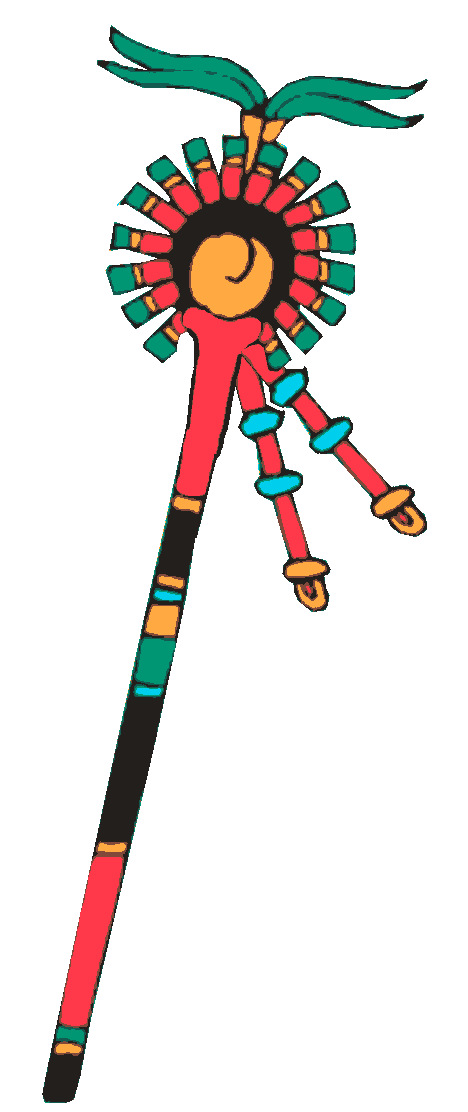
\includegraphics[height=0.3 \textheight]{Imagenes/baculo}
			\caption{Concepto de arma de Xólotl.}
			\label{fig:AtardecerVenus}
		\end{figure}
	\subsection{Portador}
	Xólotl.
%=================================================
\section{Nombre: Matlalpapalotl.}\label{Arma:LanzaItzpapalotl}
	\subsection{Descripción}
		Tepoztopilli hecho de obsidiana. Arma creada por Iztpápalotl a partir de las almas de los enemigos derrotados durante la guerra contra los dioses del norte. Es un arma de gran poder, es ligera, ideal para el combate aéreo.
	\subsection{Imagen}
		Ver figura \ref{fig:matlalpapalotl}.
			\begin{figure}
				\centering
				
\includegraphics[height=0.08 \textheight]{Imagenes/lanza02}
				\caption{Concepto de arma de Iztpápalotl.}
				\label{fig:matlalpapalotl}
			\end{figure}
	\subsection{Portador}
		Itzpápalotl.
%=================================================
\section{Nombre: Trepa viento.}\label{Arma:EspadaMictlecayotl}
\subsection{Descripción}
Macuahuitl creada por Mictlecayotl para canalizar su energía de viento y generar poderoso ataques.
\subsection{Imagen}
Ver figura \ref{fig:trepaViento}.
\begin{figure}
				\centering
				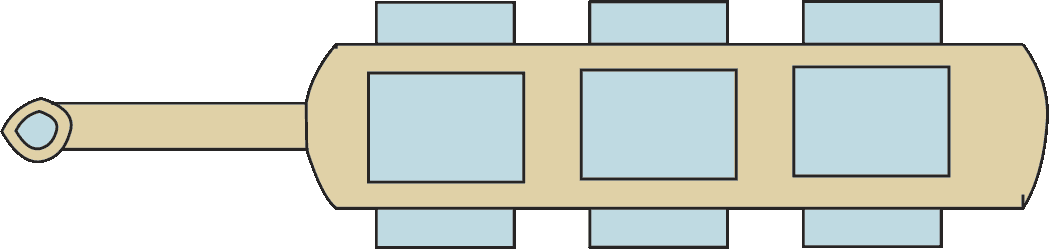
\includegraphics[height=0.1 \textheight]{Imagenes/espada}
				\caption{Concepto de arma de Mictlecayotl.}
				\label{fig:trepaViento}
\end{figure}
\subsection{Portador}
Mictlecayotl.
%=================================================
\section{Nombre: Arco solar.}\label{Arma:ArcoItztla}
\subsection{Descripción}
Arma legendaria que Itztlacoliuhqui usaba desde antes del quinto Sol, siendo éste el único objeto que se le permiti conservar de su antigua identidad. Es un arco de gran alcance, permite disparar flechas con la capacidad de destruir mundos enteros. 
\subsection{Imagen}
			Ver figura \ref{fig:ArcoSolar}.
		\begin{figure}
			\centering
			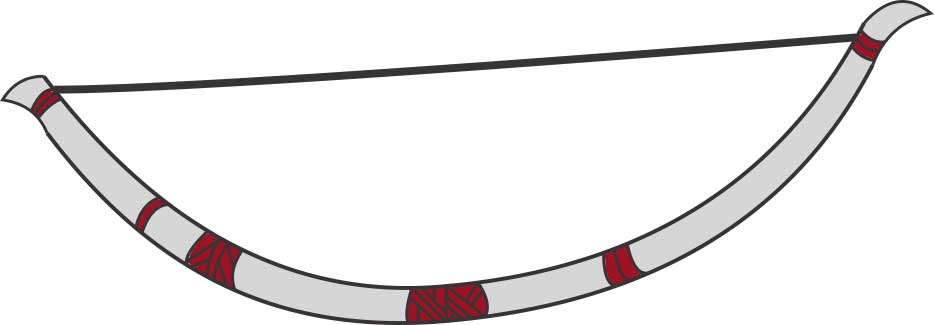
\includegraphics[height=0.1 \textheight]{Imagenes/arco}
			\caption{Concepto de arma de Itztlacoliuhqui.}
			\label{fig:ArcoSolar}
		\end{figure}
\subsection{Portador}
Itztlacoliuhqui.